\chapter{Ewaluacja aplikacji}

Za Wikipedia org 
\begin{quote}
	\textls{Ewaluacja (ang. evaluate oceniać, szacować; z łac. evalesco ;stawać się,
	być zdolnym, potężnieć; i evaleo; móc, zdołać;) – systematyczne badanie wartości albo cech
	konkretnego programu, planu działania (eksperymentu) bądź obiektu (programu komputerowego,
	programu nauczania, lekarstwa, rozwiązania technicznego) z punktu widzenia przyjętych kryteriów, w
	celu jego usprawnienia, rozwoju lub lepszego zrozumienia.}
\end{quote}
Ze względu na kryterium czasu, może to być:
\begin{itemize}
	\item ewaluacja wstępna / szacunkowa,
	\item ewaluacja ad hoc / bieżąca lub ciągła,
	\item ewaluacja ex-post / końcowa.
\end{itemize}
W naszym przypadku, z uwagi na to, że aplikacja jest już gotowa, będzie to ewaluacja „ex-post”. \newline
Ze względu na sposób prowadzenia badania rozróżniamy:
\begin{itemize}
	\item ewaluacje wewnętrzne
	\item ewaluacje zewnętrzne
\end{itemize}

\section{Plan badania}
Zastosowano ewaluację zewnętrzną, czyli powołano dwa pięcioosobowe zespoły projektowe z
jednej z zaprzyjaźnionych wrocławskich firm informatycznych, które wykorzystały naszą aplikację do
przeprowadzenia dwóch rozgrywek Planning Pokera, w celu estymacji zestawu historyjek stworzonych dla
celów testowych tylko dla tego projektu. Jeden zespól spotkał się w siedzibie firmy w sali konferencyjnej,
natomiast drugi zespól przeprowadził rozgrywkę zdalnie korzystając z komunikatora internetowego Microsoft
Lync. Oba zespoły w celu przeprowadzenia rozgrywki korzystały z naszej aplikacji.
\section{Metoda badania}
Po zakończeniu obu rozgrywek poproszono uczestników o wypełnienie stosownych ankiet.
Ankiety zostały opracowane zgodnie ze Skalą Użyteczności Systemu (System Usability Scale, SUS).
Skala ta została wymyślona przez Johna Brooke'a, który w 1986 roku stworzył szybką skalę użyteczności, aby
ocenić praktycznie każdy rodzaj systemu. \newline
SUS został wypróbowany i przetestowany przez prawie 30 lat użytkowania i sprawdził się jako
niezawodna metoda oceny użyteczności systemów w porównaniu do standardów branżowych. \newline
SUS składa się 10 pytań oraz 5 stopniowej skali ocen (opartej o skalę Likerta):
\begin{enumerate}
	\item Będę często korzystał z systemu.
	\item System jest niepotrzebnie skomplikowany.
	\item System jest łatwy w użyciu.
	\item Będę potrzebował wparcia technicznego, aby korzystać z systemu.
	\item Różne funkcje systemu są łatwo dostępne.
	\item W systemie jest zbyt wiele niespójności.
	\item Większość osób będzie w stanie opanować system bardzo szybko.
	\item System jest kłopotliwy w użyciu.
	\item Czuję się bardzo pewnie korzystając z systemu.
	\item Musiałem opanować wiele rzeczy przed rozpoczęciem pracy z systemem.
\end{enumerate}

\subsection{Jak obliczyć SUS}
Po zebraniu wyników przechodzimy do kolejnego kroku, w którym obliczamy wskaźnik SUS. Wynik
testu określany jest w punktach na skali od 0 do 100. \newline
Krok 1. Przyporządkowujemy do każdej odpowiedzi wartości od 0 do 4, zgodnie ze schematem podanym
poniżej. \newline
\newline
dla pytań 1, 3, 5, 7, 9 należy przypisać następującą punktację :
\begin{itemize}
	\item Zdecydowanie nie zgadzam się = 0
	\item Raczej nie zgadam się = 1
	\item Nie mam zdania = 2
	\item Raczej zgadzam się = 3
	\item Zdecydowanie zgadzam się = 4
\end{itemize}
dla pytań 2, 4, 6, 8, 10 punktacja wygląda następująco :
\begin{itemize}
	\item Zdecydowanie nie zgadzam się = 4
	\item Raczej nie zgadam się = 3
	\item Nie mam zdania = 2
	\item Raczej zgadzam się = 1
	\item Zdecydowanie zgadzam się = 0
\end{itemize}
Krok 2. Sumujemy punkty i mnożymy otrzymaną wartość przez 2.5.
Wynik powinien mieścić się w przedziale 0 - 100.
\subsection{Jak interpretować SUS}
Im większy wynik tym lepsza użyteczność. Wartości powyżej 68 są interpretowane jako dobry wynik,
natomiast wynik równy lub większy od 80,3 to wynik bardzo dobry. Z kolei wynik 51 lub niższy oznacza, że
użyteczność aplikacji jest niewystarczająca i koniecznie trzeba nad nią popracować.
\section{Wyniki testów}
Wyniki przeprowadzonych ankiet przedstawione zostały w tabelach 8.1 i 8.2 - jedna dotyczy zespołu,
który zebrał się w sali konferencyjnej, druga dotyczy zespołu wirtualnego (zdalnego).
Przyglądając się wynikom ankiet wg. System Usability Scale (SUS), można zauważyć, że zespól zdalny
ocenił aplikację nieco gorzej, bo na 77 punktów rys:\ref{rys:badanie2}, natomiast zespół „bliski” na 83,5 punktów. Daje to
średni wynik 80,25, czyli prawie 80,3. Rys: \ref{rys:badanie1}
Można powiedzieć, że w tym szybkim badaniu osiągnęliśmy wynik bardzo dobry. Warto jednak
bardziej szczegółowo przeanalizować wyniki ankiet. Można zauważyć, że zarówno jeden, jak i drugi
zespół projektowy przyznał mniej punktów odpowiadając na pytania 2, 6 i 8:
\begin{itemize}
	\item 2. System jest niepotrzebnie skomplikowany.
	\item 6. W systemie jest zbyt wiele niespójności.
	\item 8. System jest kłopotliwy w użyciu
\end{itemize} 

\begin{figure}[H]
	\centering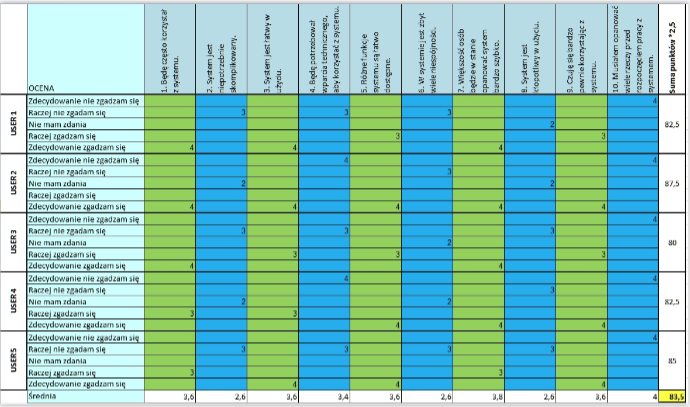
\includegraphics[width=\textwidth]{img/Badanie1.png}
	\caption{Tablica wyników ankiet SUS dla zespołu „bliskiego”.}\label{rys:badanie1}% Źródło rysunku i etykieta przez którą odwołujemy się do rysunku.
\end{figure}

Znalazło to potwierdzenie w rozmowie z uczestnikami badania, którzy podnosili następujące kwestie:
\begin{itemize}
	\item Niezbyt wygodny ekran, ponieważ wymaga skrolowania.
	\item Niespójny interfejs.
	\item Zbyt dużo kroków do rozpoczęcia nowej gry.
	\item Nie można stworzyć backloga do gry za pomocą tekstowego filtra.
	\item Brak szczegółowej instrukcji.
	\item Brak pomocy.
\end{itemize}
Badani stwierdzili, iż aplikacja spełnia założony cel. Wymaga ona jeszcze dopracowania. Jednak dzięki
swoim unikatowym cechom może znaleźć grupę docelową.
Zespół zaznaczył, że w sposób podobny oceniają swoje historyjki w postaci etykiet na GitHub, jednak
robią to ręcznie. Głosowanie odbywa się wtedy przy użyciu komunikatora, jednak jest to bardzo czasochłonne i
zdarzają się problemy. Uczestnicy badania stwierdzili, że takie narzędzie z pewnością ułatwiłoby im estymacje.
Po wynikach ankiet widać, że aplikacja wymaga jeszcze dopracowania. Problemem jest nawigacja po
aplikacji, gdyż wymaga zbyt wielu przejść do ekranów by rozpocząć grę. Członkowie najchętniej zaczęliby grę,
wpisując w pole tekstowe nazwę repozytorium, a w drugie odpowiednie filtry by zacząć grę. W aplikacji nie ma
też zbyt wielu przydatnych objaśnień. Według jednego z programistów sam formularz ustawień gry powinien
być trochę przeprojektowany, aby wiadomo było, jakie pola są obowiązkowe, oraz co zmieniają w całej
rozgrywce.
\begin{figure}[H]
	\centering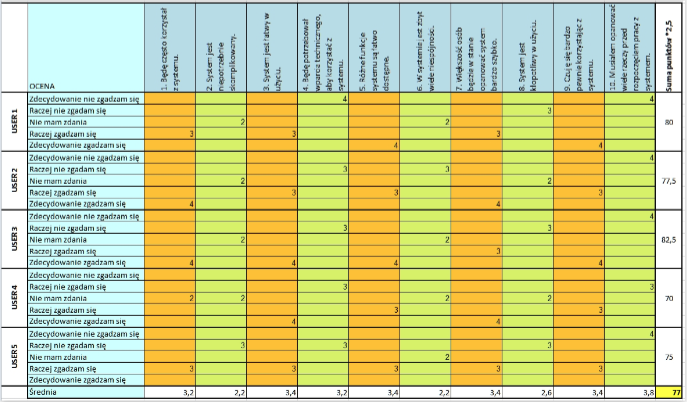
\includegraphics[width=\textwidth]{img/Badanie2.png}
	\caption{Tablica wyników ankiet SUS dla zespołuzdalnego.}\label{rys:badanie2}% Źródło rysunku i etykieta przez którą odwołujemy się do rysunku.
\end{figure}
Aplikacji przydałby się też odpowiedni dział pomocy, mówiący o tym jak grać w Planning Poker, oraz jak
należy odpowiednio estymować zadania. Mimo tego aplikacja dzięki swojej integracji z narzędziem GitHub
wyróżnia się na tle konkurencji. Jeżeli w aplikacji zostanie przeprojektowany sposób tworzenia gry na szybszy
oraz dodane trochę więcej opcji to może okazać się dość dobrym wyborem dla programistów.
Można przyznać, iż aplikacja spełnia swoje zadanie i z powodzeniem może być wykorzystana jako
narzędzie wspomagające estymację zadań projektowych metodą Planning Poker.
